\begin{activity} \label{A:9.7.4} Let
\[\vr(t) = \cos(t) \vi - \sin(t) \vj + t \vk.\footnote{You can sketch the graph with Wolfram Alpha, the applet at \url{http://gvsu.edu/s/LR}, or some other appropriate technology.}\]
    \ba
    
    \item Determine the coordinates of the point on the curve traced out by $\vr(t)$ when $t = \pi$.
    
    \item Find a direction vector for the line tangent to the graph of $\vr$ at the point where $t=\pi$.

    \item Find the parametric equations of the line tangent to the graph of $\vr$ when $t=\pi$.

    \item Sketch a plot of the curve $\vr(t)$ and its tangent line near the point where $t = \pi$.  In addition, include a sketch of $\vr'(\pi)$.  What is the important role of $\vr'(\pi)$ in this activity?

    \ea

\end{activity}
\begin{smallhint}

\end{smallhint}
\begin{bighint}

\end{bighint}
\begin{activitySolution}
    \ba
    \item Since
    \[\vr(\pi) = \cos(\pi) \vi - \sin(\pi) \vj + \pi \vk = -\vi + \pi \vk,\]
the point on the curve traced out by $\vr(t)$ when $t = \pi$ is $(-1,0,\pi)$. 
    \item The derivative 
\[\vr'(\pi) = -\sin(\pi)\vi - \cos(\pi)\vj + \vk = \vj + \vk\]
is a direction vector for the line tangent to the graph of $\vr$ at the point where $t=\pi$.
    \item Using the point and the direction vector found in (a) and (b), the parametric equations of the line tangent to the graph of $\vr$ when $t=\pi$ are
\[x(t) = -1, \ \ \ y(t) = t, \ \ \ z(t) = \pi+t.\]
    \item The sketch below shows the curve $\vr(t)$ and a direction vector $\vr'(\pi)$ for the tangent line to the curve at $t=\pi$. 
%\begin{figure}[ht]
\begin{center}
\resizebox{!}{2.0in}{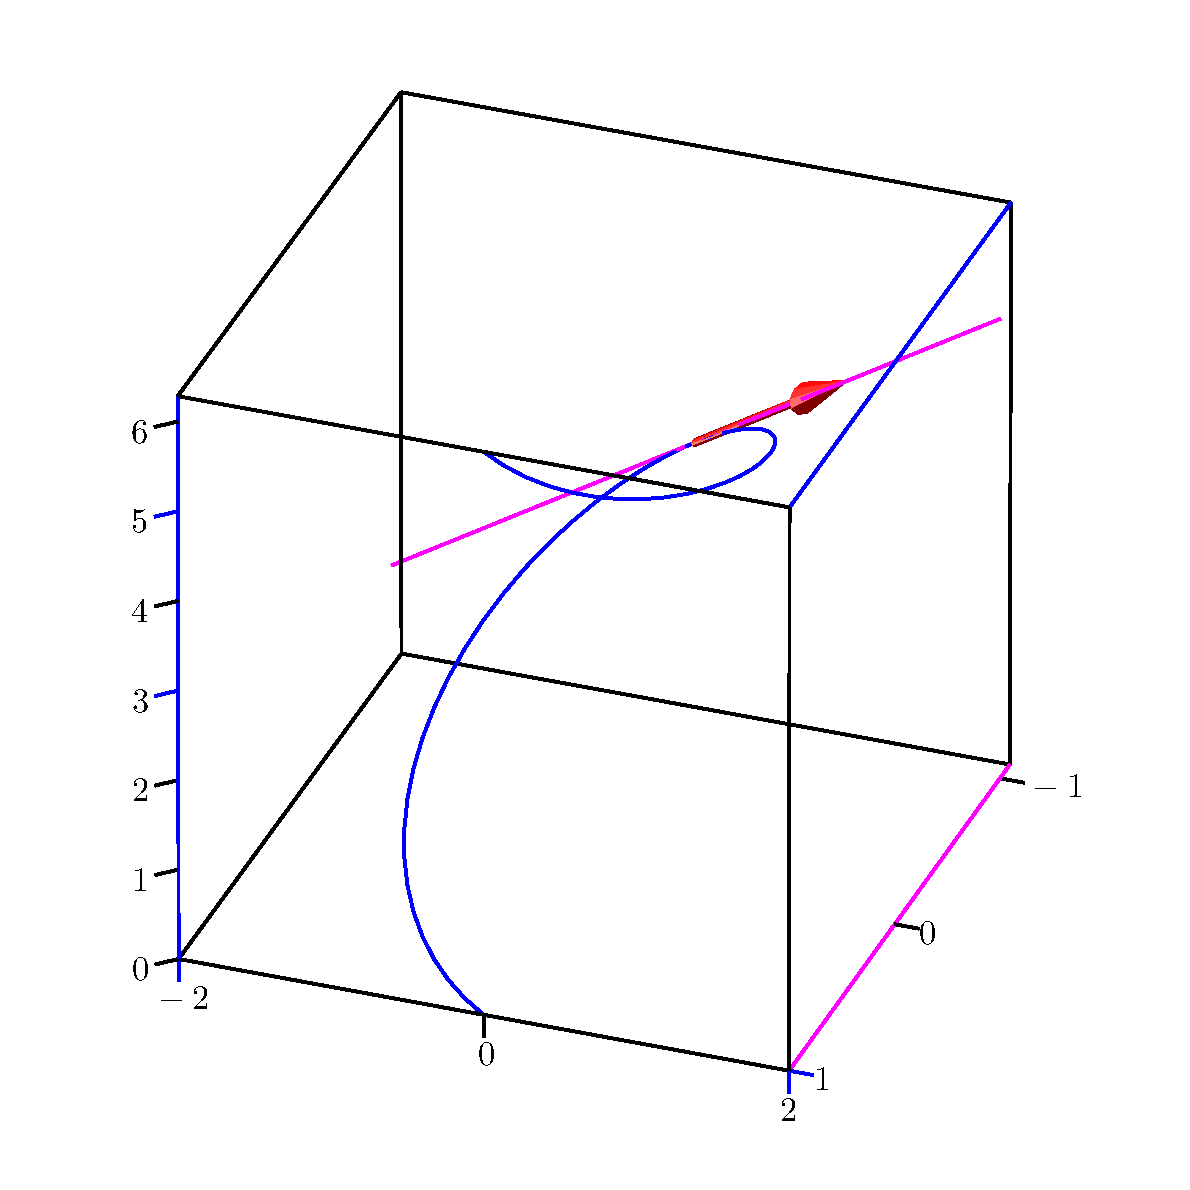
\includegraphics{figures/9_7_Act29_d_sol}}
%\caption{The distance formula in $\R^3$.}
%\label{F:9.1.Distance_3D}
\end{center}
%\end{figure}

    \ea
\end{activitySolution}
\aftera
